\chapter{Result and Discussion}\label{chap5}
\newpage
\section{Implementation status}
Table~\ref{tab:status} lists every module and its status on 26 September 2026. All code is in the public repository \texttt{github.com/Rhian-Roy/DiaCausal-CDSS}; 168 automated tests (139 engine, 13 RAG, 16 website) pass on every change.
\begin{longtable}{>{\raggedright\arraybackslash}p{4.1cm}>{\raggedright\arraybackslash}p{2.2cm}>{\raggedright\arraybackslash}p{6.2cm}>{\raggedright\arraybackslash}p{1.6cm}}
\caption{Implementation status (26 September 2026)}\label{tab:status}\\\toprule
Module & Status & Evidence & Owner\\\midrule\endhead
Synthetic cohort generator & Done & \texttt{params.yaml}: every number has a source and a status; tests & Rhian\\
Safety rules (\texttt{rules.csv}) & Done & 10 cited rules (7 verified against labels, 3 team-set cut-offs flagged for the clinician); tests & Rhian\\
Propensity model and overlap check & Done & Cross-fitted multinomial model; overlap figure; tests & Rhian\\
Naive, IPW, matching and AIPW & Done & Results table; 95\% intervals; tests & Rhian\\
DR-learner (patient-level effects) & Done & Recovery and calibration figures; S- and T-learner baselines & Rhian\\
Benchmark, metrics, refutation, E-values & Done & \texttt{results/}: 20 cohorts $\times$ 5{,}000 patients; 9/9 refutation checks pass & Rhian\\
Demo (Streamlit) and FastAPI endpoint & Done & \texttt{POST /api/v1/recommend}; screenshots & Rhian\\
Phone website (installable, offline) & Done & \url{https://diacausal.netlify.app}; browser and Python give identical answers (155 patients) & Rhian, Graceton\\
Accounts: sign-up, authenticator app, admin approval & Done & Row-level security; tested end to end & Rhian\\
Chat application (sign-in, guards, patient panel, voice) & Done (separate) & Engine integration planned for October & Team\\
RAG retrieval with citations & In progress & Licence gate, chunking, BM25 + vector + fusion; first FDA source; Evidence tab & Rhian\\
Hypoglycaemia and weight outcomes; consultation summary & In progress & Target 9 October & Rhian\\
RAG explanation writer, gold questions, evaluation & Planned & 1--16 October & Team\\
Clinician vignette review and usability survey & Planned & 10--23 October & Advik\\
Research paper & Planned & After results are frozen (16 October) & Pratham\\\bottomrule
\end{longtable}

\section{Implementation}
The engine is written in Python and organised as small, separately tested modules. The generator creates an India-calibrated synthetic cohort in which doctors' prescribing depends on patient characteristics (confounding by indication) and every patient's outcome under all three drugs is stored, so the true effects are known. The safety rules module reads \texttt{rules.csv} and removes or flags options with a cited reason; thresholds are never hard-coded, and a test scans the code to prove it. The propensity module fits a five-fold cross-fitted multinomial logistic regression and flags options whose propensity is below 0.05. The estimators module computes naive, inverse probability weighted (IPW), matching and AIPW average effects with 95\% confidence intervals, and a DR-learner with robust intervals for patient-level effects. The metrics module compares every estimate with the known truth. A benchmark script repeats the whole process on 20 simulated cohorts and writes the results table and figures used below. A Streamlit demo, a FastAPI endpoint and the phone website expose the same pipeline, and each reply is checked for the intended-use statement and for dose-like text before it is shown.

\section{Initial results}
All results in this section come from the synthetic cohort, where the true effects are known. They show whether the methods recover the truth; they do not show clinical validity on real patients.
\begin{table}[H]\centering\small
\caption{Synthetic benchmark results: 20 cohorts of 5{,}000 patients, with 2{,}000 fresh test patients each}\label{tab:results}
\resizebox{\textwidth}{!}{\parbox{22.5cm}{\centering% DiaCausal causal engine v0.3.0 benchmark: 20 synthetic cohorts x 5000 patients.
% SYNTHETIC DATA ONLY. Made by the benchmark script (see README); do not edit by hand.
\begin{tabular}{llrrrr}
\hline
Contrast & Method & Truth & Bias & RMSE & 95\% CI coverage \\
\hline
SGLT2i vs DPP-4i & naive & $-0.211$ & $-0.159$ & 0.160 & 0.00 \\
SGLT2i vs DPP-4i & IPW & $-0.211$ & 0.001 & 0.022 & 1.00 \\
SGLT2i vs DPP-4i & matching & $-0.211$ & $-0.002$ & 0.026 & 0.95 \\
SGLT2i vs DPP-4i & AIPW & $-0.211$ & 0.002 & 0.023 & 0.95 \\
\hline
Sulfonylurea vs DPP-4i & naive & $-0.256$ & $-0.106$ & 0.108 & 0.00 \\
Sulfonylurea vs DPP-4i & IPW & $-0.256$ & $-0.004$ & 0.025 & 1.00 \\
Sulfonylurea vs DPP-4i & matching & $-0.256$ & $-0.008$ & 0.028 & 1.00 \\
Sulfonylurea vs DPP-4i & AIPW & $-0.256$ & $-0.003$ & 0.027 & 0.95 \\
\hline
SGLT2i vs Sulfonylurea & naive & 0.045 & $-0.052$ & 0.056 & 0.50 \\
SGLT2i vs Sulfonylurea & IPW & 0.045 & 0.005 & 0.030 & 0.95 \\
SGLT2i vs Sulfonylurea & matching & 0.045 & 0.006 & 0.026 & 0.95 \\
SGLT2i vs Sulfonylurea & AIPW & 0.045 & 0.005 & 0.030 & 0.90 \\
\hline
\end{tabular}

\vspace{1em}

\begin{tabular}{lrrrr}
\hline
Learner & PEHE SGLT2i vs DPP-4i & PEHE Sulfonylurea vs DPP-4i & PEHE SGLT2i vs Sulfonylurea & Policy regret \\
\hline
DR-learner & 0.105 & 0.117 & 0.108 & 0.011 \\
T-learner & 0.189 & 0.192 & 0.184 & 0.029 \\
S-learner & 0.103 & 0.104 & 0.110 & 0.012 \\
naive & 0.214 & 0.197 & 0.169 & 0.062 \\
\hline
\end{tabular}
}}
\end{table}
The true effects are $-0.211$ (SGLT2i minus DPP-4i), $-0.256$ (sulfonylurea minus DPP-4i) and $+0.045$ (SGLT2i minus sulfonylurea) HbA1c percentage points. The naive comparison overstates the SGLT2i-versus-DPP-4i benefit by about 75\% ($-0.370$ against $-0.211$) and its intervals never contain the truth, because sicker patients received SGLT2i more often. IPW, matching and AIPW remove almost all of this bias ($|\text{bias}|\le 0.008$) with 90--100\% interval coverage. For individual patients, the DR-learner's error (PEHE 0.105--0.117) is about half the T-learner's and similar to the S-learner's, but unlike either it gives every patient a 95\% interval, which contained the true patient effect for 94.4\%, 94.7\% and 92.7\% of test patients. Choosing the option with the lowest DR-learner estimate lost on average 0.011 HbA1c points against perfect knowledge (policy regret), compared with 0.062 for the naive averages. The system answered ``insufficient evidence'' or ``excluded'' for 2.5\% of patient--option pairs. After weighting, the largest standardised mean difference fell from 0.70 to 0.08, below the 0.1 balance threshold \cite{austin2009}. All nine refutation checks passed (placebo treatment, random common cause and 80\% subsets for each contrast), and the E-values were 1.57--2.15 for the estimates.
\begin{figure}[H]\centering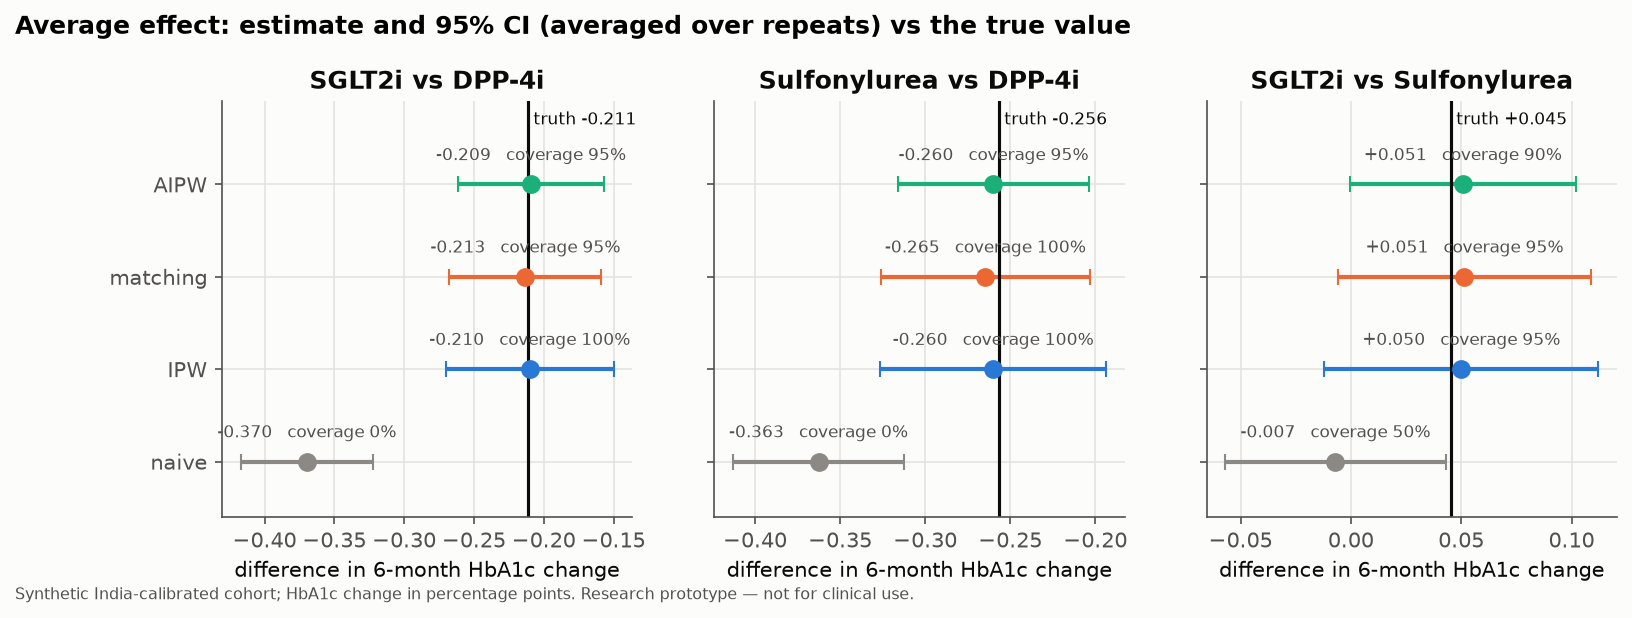
\includegraphics[width=0.9\textwidth]{results/figures/ate_vs_truth.png}
\caption{Estimated versus true average effect for the naive, IPW, matching and AIPW methods across repeated cohorts}\label{fig:ate}\end{figure}
\begin{figure}[H]\centering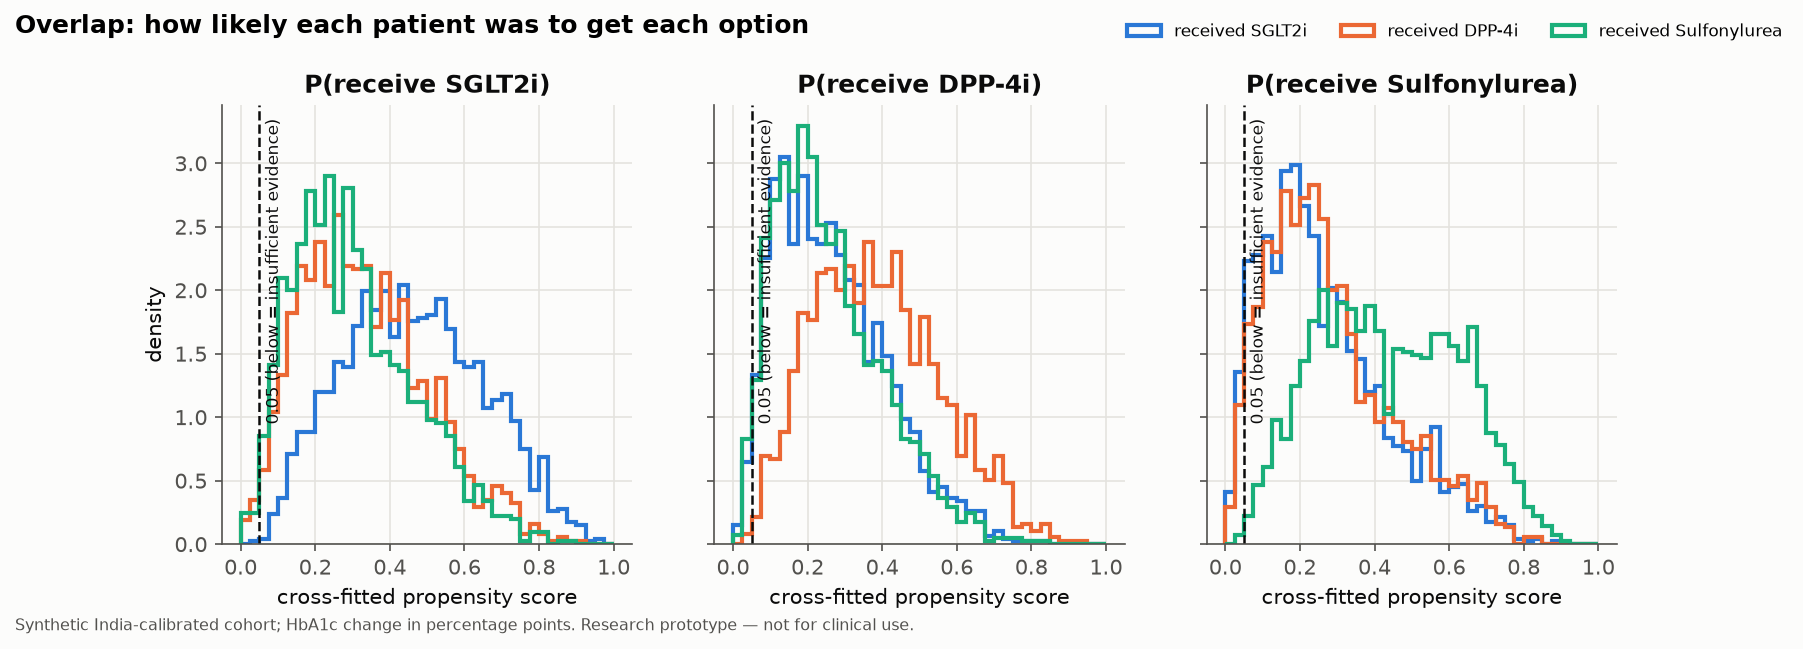
\includegraphics[width=0.9\textwidth]{results/figures/overlap.png}
\caption{Propensity overlap for each drug; the dashed line marks the 0.05 abstention threshold}\label{fig:overlap}\end{figure}
\begin{figure}[H]\centering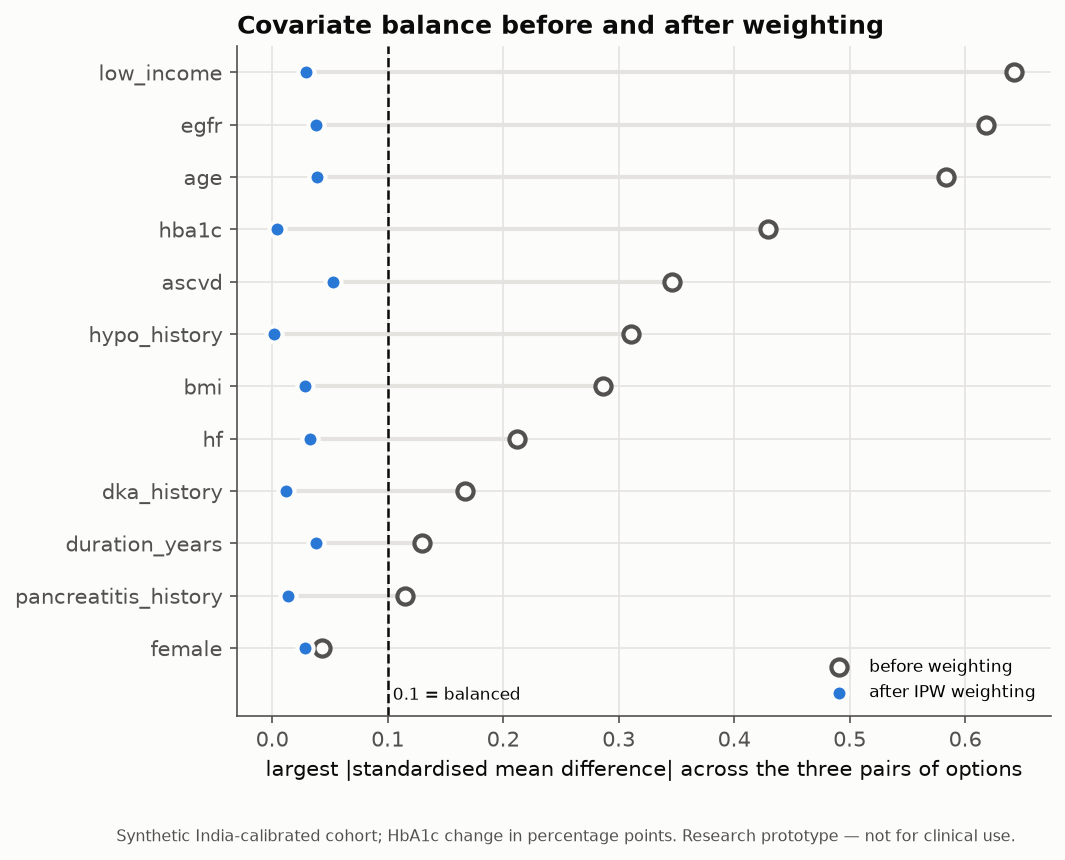
\includegraphics[width=0.8\textwidth]{results/figures/love_plot.png}
\caption{Covariate balance before and after weighting (target: standardised difference below 0.1 \cite{austin2009})}\label{fig:love}\end{figure}
\begin{figure}[H]\centering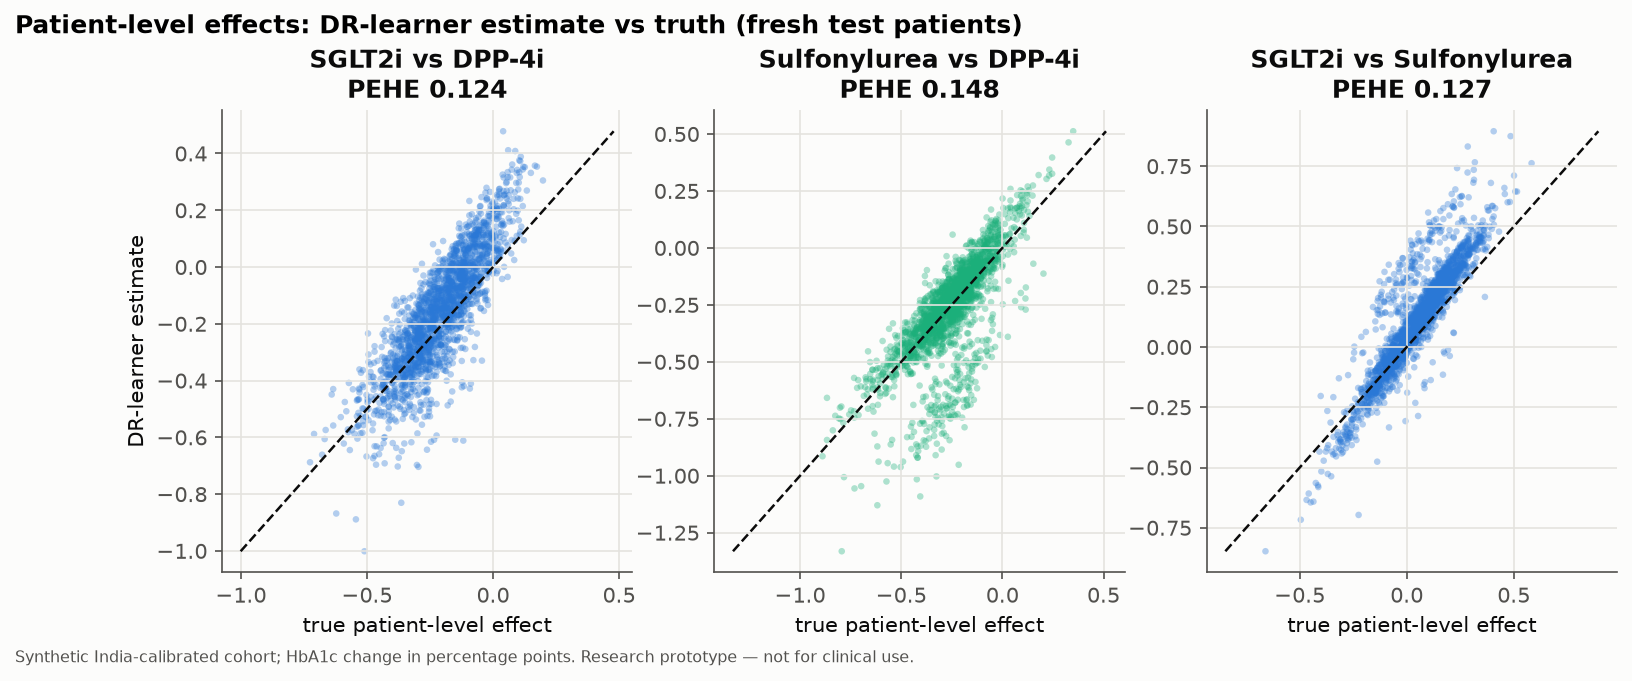
\includegraphics[width=0.9\textwidth]{results/figures/cate_recovery.png}
\caption{Patient-level effects estimated by the DR-learner against the true effects}\label{fig:cate}\end{figure}
\begin{figure}[H]\centering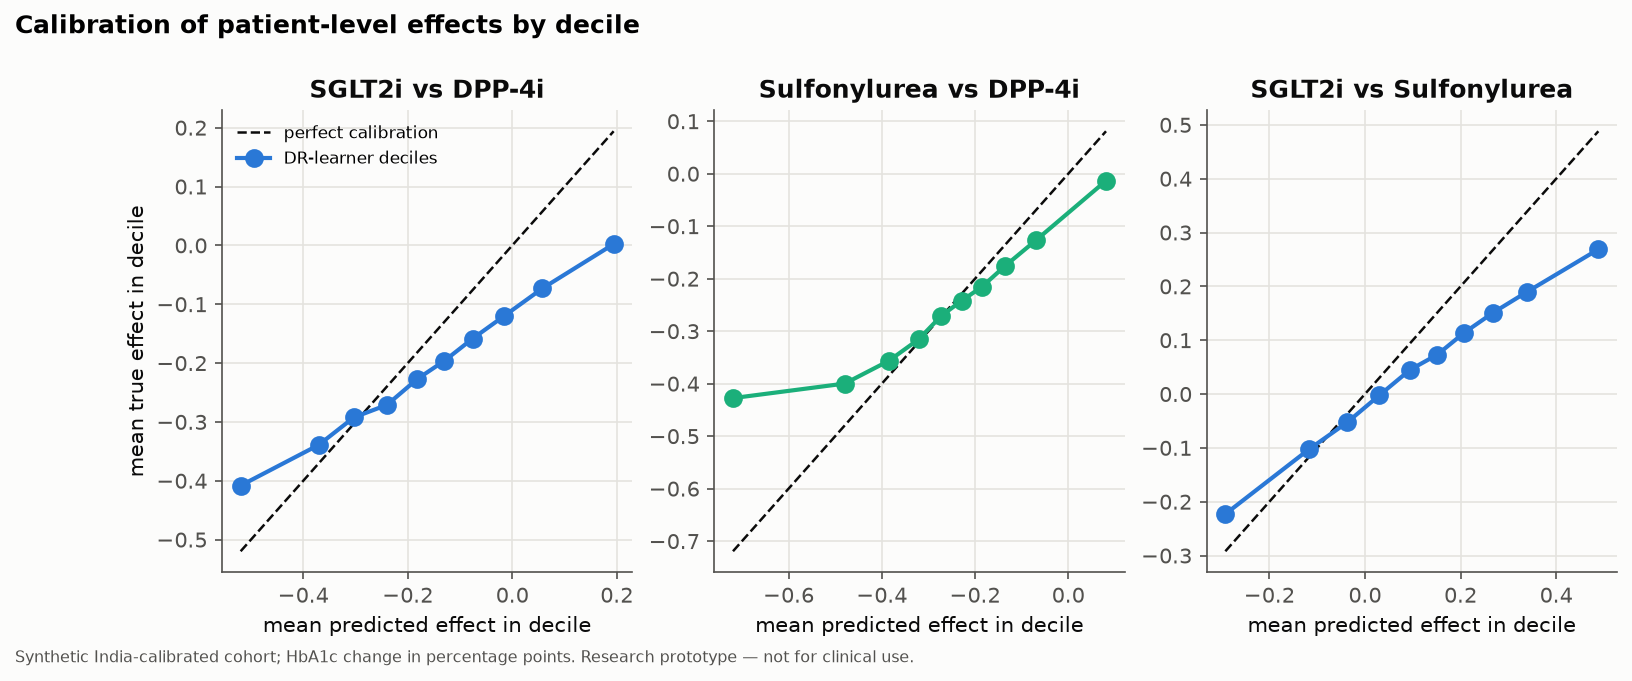
\includegraphics[width=0.9\textwidth]{results/figures/calibration.png}
\caption{Calibration of patient-level effect estimates by decile}\label{fig:calib}\end{figure}

\section{Screenshots of the System}
\begin{figure}[H]\centering
\includegraphics[width=0.78\textwidth]{screens/demo1.png}
\caption{Demo: a typical patient with an estimate and 95\% range for each option}\label{fig:demo1}\end{figure}
\begin{figure}[H]\centering
\includegraphics[width=0.78\textwidth]{screens/demo2.png}
\caption{Demo: an exclusion and cautions with their sources (eGFR 40, history of pancreatitis)}\label{fig:demo2}\end{figure}
\begin{figure}[H]\centering
\includegraphics[width=0.78\textwidth]{screens/demo3.png}
\caption{Demo: ``insufficient evidence'' shown instead of a guess (older patient, past hypoglycaemia)}\label{fig:demo3}\end{figure}
\begin{figure}[H]\centering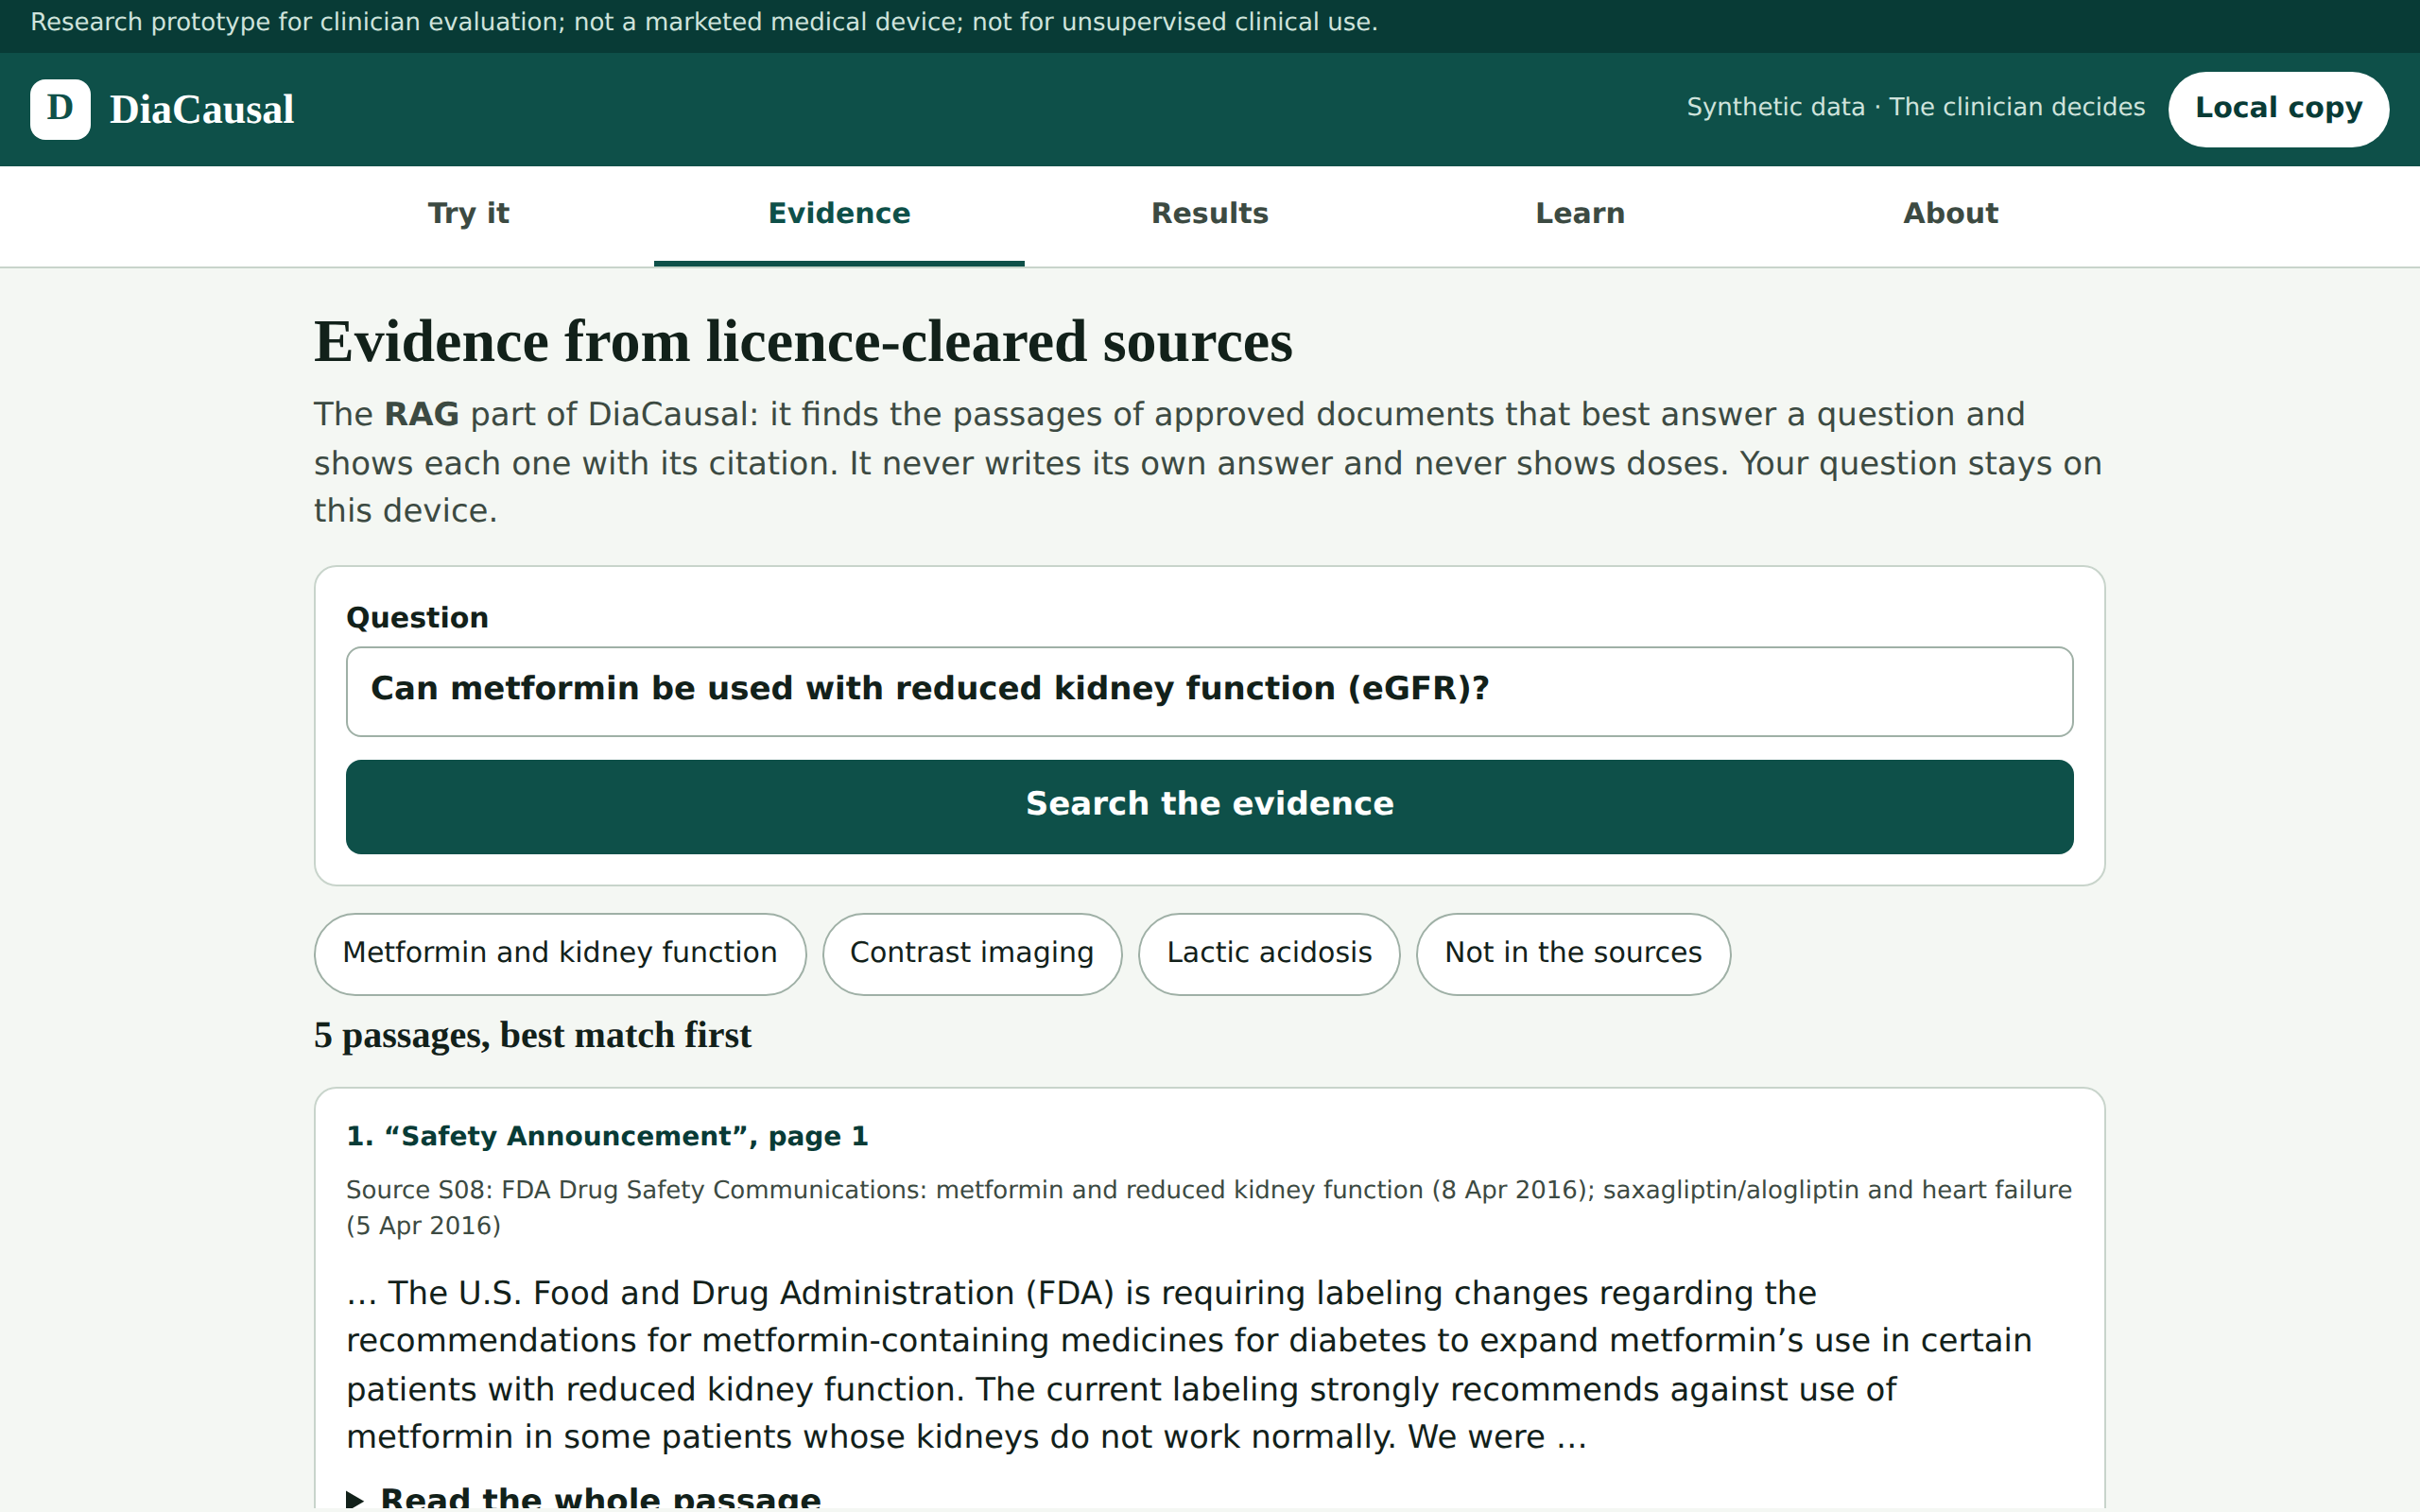
\includegraphics[width=0.9\textwidth]{screens/evidence_desktop.png}
\caption{Evidence tab: cited passages from a licence-cleared source (early RAG retrieval)}\label{fig:evidence}\end{figure}
\begin{figure}[H]\centering
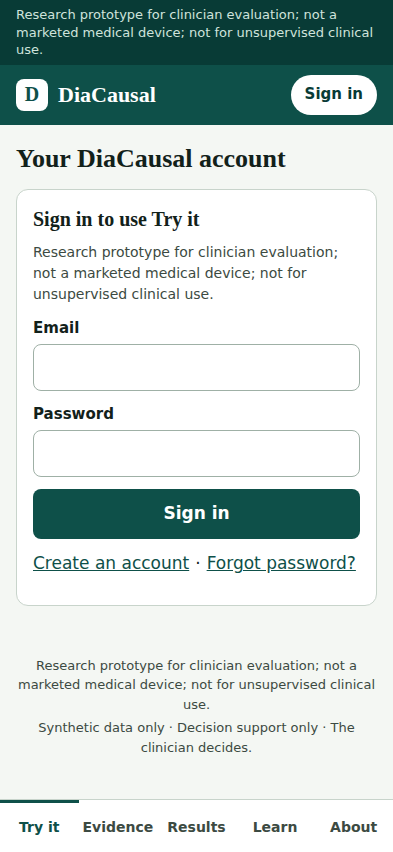
\includegraphics[height=8.5cm]{screens/signin_phone.png}\hspace{1cm}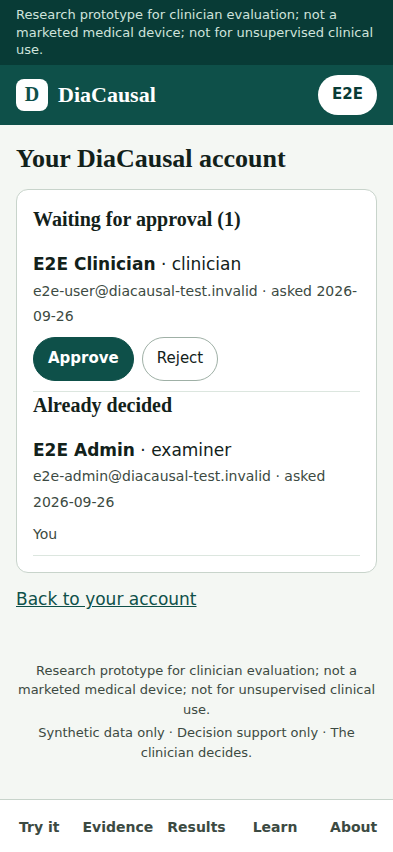
\includegraphics[height=8.5cm]{screens/admin_phone.png}
\caption{Phone website: sign-in (left) and the admin's approval screen with test accounts (right)}\label{fig:phone}\end{figure}

\section{Sample Code (implementation)}
The listings below are copied from the project repository (\texttt{diacausal\_engine/}).
\lstinputlisting[caption={Safety rules engine (guardrails.py): rules are read from rules.csv, never hard-coded},firstline=35,lastline=101]{code/guardrails.py}
\lstinputlisting[caption={AIPW scores (estimators.py)},firstline=163,lastline=175]{code/estimators.py}
\lstinputlisting[caption={DR-learner with HC3 robust intervals (estimators.py)},firstline=194,lastline=231]{code/estimators.py}

\section{Evaluation matrix}
Table~\ref{tab:eval} lists how the complete system will be judged. Targets marked L come from the literature; targets marked T were set by the team. The last column gives the mid-semester result where one exists (synthetic data).
\begin{longtable}{>{\raggedright\arraybackslash}p{1.6cm}>{\raggedright\arraybackslash}p{2.5cm}>{\raggedright\arraybackslash}p{3.1cm}>{\raggedright\arraybackslash}p{2.4cm}>{\raggedright\arraybackslash}p{3.5cm}}
\caption{Evaluation matrix}\label{tab:eval}\\\toprule
Part & Metric & Meaning & Target & Mid-semester result\\\midrule\endhead
Causal & PEHE per drug pair & Error of patient-level effects & Lower than simple learners (T) & DR 0.105--0.117 vs T-learner 0.184--0.192; naive 0.169--0.214 \\
Causal & Bias and RMSE of average effects & Over repeated cohorts & $|$bias$|\le 0.1$ at $n=5{,}000$ (T) & AIPW $|$bias$|\le 0.005$; RMSE 0.023--0.030 \\
Causal & 95\% interval coverage & Share of intervals containing the truth & 90--97\% (T) & AIPW 90--95\%; DR-learner 92.7--94.7\% \\
Causal & Policy regret & Loss from choosing the estimated best option & Lower than naive (T) & 0.011 vs 0.062 \\
Causal & Covariate balance & Largest SMD after weighting & Below 0.1 (L \cite{austin2009}) & 0.70 $\rightarrow$ 0.08 \\
Causal & Overlap and abstention & Share of answers refused & Reported (T) & 2.5\% of patient--option pairs \\
Causal & Refutation tests & Placebo, random cause, subsets & Placebo near 0; stable (L \cite{dowhy}) & 9/9 passed \\
Causal & E-value & Strength of hidden confounding needed & Reported (L) & 1.57--2.15 \\
Safety rules & Rule tests & Rules unit-tested and passing & 100\% (T) & 100\% (168 tests pass) \\
Safety rules & Unsafe options shown & On 50 or more test cases & 0 (T) & 0: an excluded option is never estimated (checked on 155 test patients); formal set in October \\
RAG & Recall@5 & Right passage in the top 5 & At least 0.80 (T) & October (gold questions) \\
RAG & Citation precision & Citations that support the sentence & At least 0.95 (T) & October \\
RAG & Faithfulness & Claims supported by passages & At least 0.90 (T) & October (RAGAS \cite{es2024}) \\
RAG & Abstention accuracy & Out-of-scope questions refused & At least 0.95 (T) & October \\
RAG & Free-text doses & Doses written by the system & 0 (T) & 0 (dose check on every reply) \\
Clinician & Agreement & Cohen's $\kappa$ on 60 cases & At least 0.61 (L \cite{landis1977}) & October (vignette study) \\
Clinician & Usability & System Usability Scale & At least 68 (L \cite{brooke1996}) & October (survey) \\
System & Latency & 95th-percentile response time & Under 3 s (T) & Website answers on the device instantly; load test in October \\
System & Audit completeness & Requests logged & 100\% (T) & Every engine request logged (tested) \\
Licences & Licence records & Sources with a licence category & 100\% (T) & 100\% (21 sources in the registry) \\\bottomrule
\end{longtable}

\section{Discussion: work completed and work planned}
By the mid-semester review the causal half of DiaCausal --- data generation, safety rules, estimation, evaluation, refutation, demo, API and a live phone website with approved accounts --- is implemented and tested on synthetic data, which is well beyond the required 25\%. Because the true effects are synthetic, good recovery shows that the estimators are correct, not that the system is valid for real patients; that is why a clinician review and a real-data check are part of the plan. The remaining work, scheduled before 30 October 2026, is the secondary outcomes and consultation summary, the RAG layer with cited explanations and its evaluation, integration of the engine with the chat application, the full evaluation in Table~\ref{tab:eval}, the clinician review, and the research paper.
